\documentclass[12pt, letterpaper]{article}
\usepackage[utf8]{inputenc}
\usepackage{bera}
\usepackage{titling}
\renewcommand\maketitlehooka{\null\mbox{}\vfill}
\renewcommand\maketitlehookd{\vfill\null}
\usepackage{graphicx}
\graphicspath{ {./images/} }


\title{\textbf{\Huge Wireless-X \\
\LARGE CS699 Software Lab Project\\
\LARGE Indian Institute of Technology, Bombay}}
\date{\Large 17th November, 2020}
\author{\LARGE PARA-Site\\
\textbf{Rajneesh Katkam} \\ 203050086\\
\textbf{Aditya Pradhan} \\ 203059006\\
\textbf{Ajinkya Jumbad} \\ 203050032\\
\textbf{Prashant Ravi} \\ 203050082\\
}


\begin{document}

\maketitle
\thispagestyle{empty}
\clearpage
\pagenumbering{arabic}
\newpage

\tableofcontents
\newpage

\section{Introduction}
Covid has hit us all hard in one way or another. For us students, it has been a lot of things, like missing being on campus, taking the load of online semester in the complete absence of \textit{relaxing perks} of offline semester, managing equipment needed for online semester and compromising with our comfort (sitting on a chair, keeping your face shoved in laptop whole day is painful). While we can't do much to compensate for offline semester, we can surely devise an idea to reduce the load of managing so many equipment and restoring some of your comfort back. The materialization of this idea is a legen-- wait for it-- dary app called - \textbf{Wireless-X}. (HIMYM fans, did we get you?)

The total package of Wireless-X consist of an android app being backed by a Python server. Using this app, we have tried to eliminate the need to buy a wireless mouse, wireless keyboard and a dedicated web-cam. Instead, using this app, user can use his/her android phone's screen as his mouse, a custom build keyboard layout as his wireless keyboard and his/her smartphone's camera as web-cam. A Python server running on target laptop will capture these commands and emulate the effects on laptop. 

\section{Motivation}
The key motivation behind this idea came from one of our teammate who, despite owning an amazing gaming rig, did not have a web-cam and had to buy one for remote proctored midsems (Yes, he is in 2020 and don't use a laptop). This, in our opinion, was an unnecessary expense. And we realised that this problem isn't limited to our teammate only and in fact affect a wider range of people and not just students. 

People come from different economical background and buying a wireless mouse, or keyboard or web-cam may not be easy for everyone. And even if they can manage to buy one, it is not efficient to do so when they have already invested on a smartphone. One thing, that is very common now-a-days across all section of society is having a smartphone, either a basic or a high-end one doesn't matter. 

The required hardware to emulate a wireless keyboard, mouse or external web-cam is already present in a smartphone, and we just need to tailor it to make it usable for a common end-user. \textbf{Rajneesh}, our teammate, came up with this idea of Wireless-X where he proposed that we can use smartphone's hardware via an app to compensate for these three devices.

\section{End-User Documentation}
\textbf{NOTE:} This user manual has been written with an assumption that end user is running Linux based OS. For Windows, few setup step will differ but writing a user manual for Windows will be a future scope. Also, the current git repository is private and maintained on git.cse.iitb.ac.in so setup steps are written keeping this in mind so TAs while checking can easily naivgate through setup process. Changes for a general end-user will differ slightly but we won't be capturing it for the time being.
\subsection{Laptop Side (Python Server)}
\begin{enumerate}
    \item On your laptop, open terminal by pressing Ctrl+Alt+T.
    \item Type \textbf{git clone https://git.cse.iitb.ac.in/rajneeshkatkam/PARA-Site\_WirelessX} in your terminal and hit enter. It will ask for your gitcse username.
    \begin{center}
    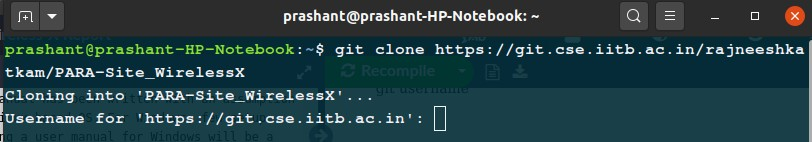
\includegraphics[scale=0.5]{images/gitclone.jpg}
    \end{center}
    \item Enter your username and password. Let the repository clone. Once cloned, the terminal will look like this:
    \begin{center}
    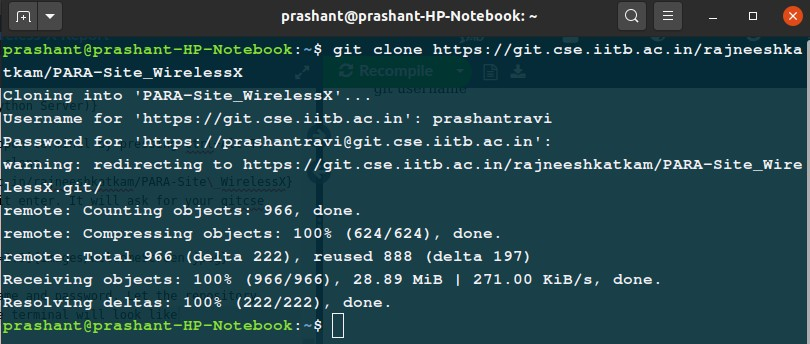
\includegraphics[scale=0.5]{images/cloned.jpg}
    \end{center}
    \item Type \textbf{cd PARA-Site\_WirelessX/source/WirelessX-Python-Server/} in your terminal. Your current working directory will change to above mentioned path. Please refer below image:
    \begin{center}
    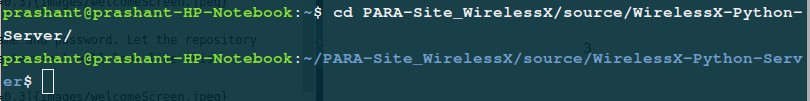
\includegraphics[scale=0.5]{images/cdDir.jpg}
    \end{center}
    \item Type \textbf{sudo chmod a+x install.sh} in your terminal and hit enter. It will ask for your system password. Please enter it.
    \begin{center}
    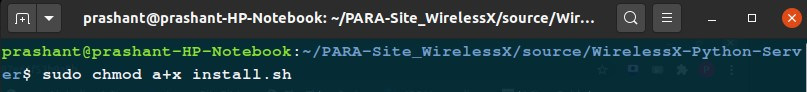
\includegraphics[scale=0.5]{images/chmod.jpg}
    \end{center}
    \item Type \textbf{sudo ./install.sh} in your terminal and hit enter. It will install all required dependencies.
    \begin{center}
    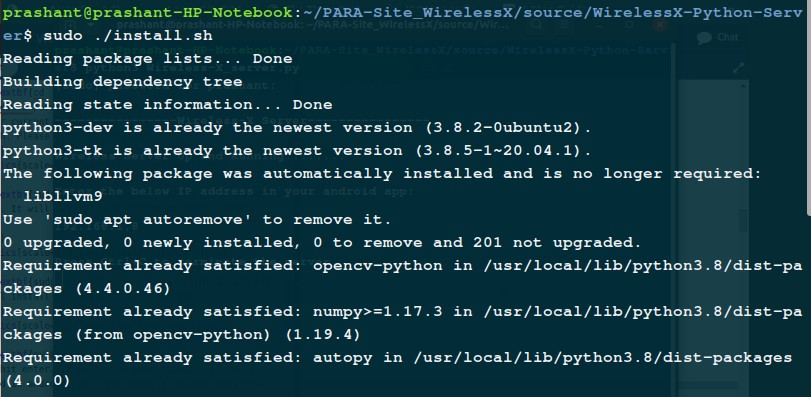
\includegraphics[scale=0.5]{images/install.jpg}
    \end{center}
    \item Type \textbf{python3 Wireless-X\_server.py} in your terminal and hit enter. It will show your laptop's IP which will be needed in android app. Your terminal should look like this:
    \begin{center}
    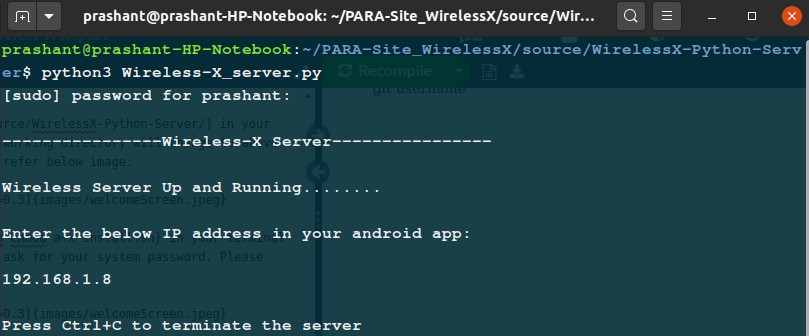
\includegraphics[scale=0.5]{images/server.jpg}
    \end{center}
\end{enumerate}
\subsection{Smartphone Side (Android App)}
\begin{enumerate}
\item Get the apk from source directory and install it in your android smartphone. You may have to grant permission to install from unknown resources. 
\item Once installed, open the app. Welcome screen should be like this:
\begin{center}
    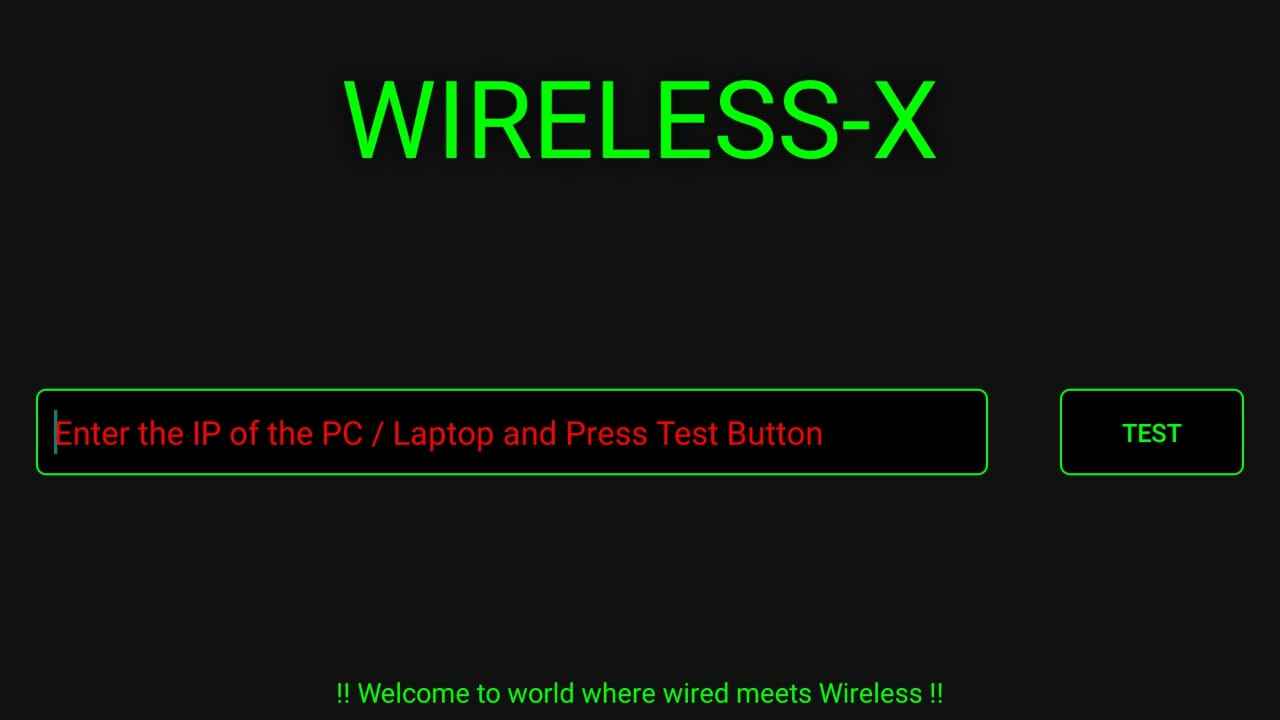
\includegraphics[scale=0.25]{images/welcomeScreen.jpeg}
\end{center}
\item Make sure that your laptop and mobile phone are on same network. Suggested way is connect your laptop to your mobile hotspot.
\item Enter your laptop IP (which is being showed in your terminal where you are running Wireless-X server) in Wireless-X app on your phone. 
\item If connection is successful, following screen will appear:
\begin{center}
    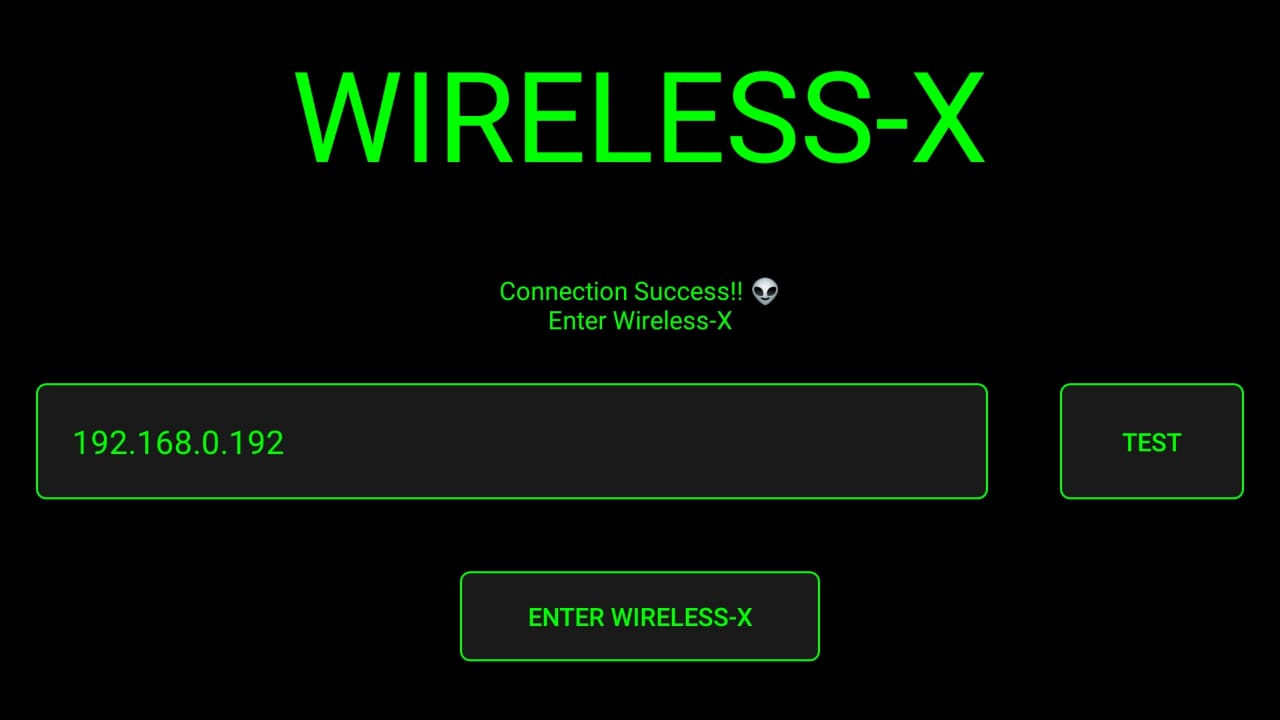
\includegraphics[scale=0.25]{images/connectionSuccessful.jpeg}
\end{center}
\item If connection is unsuccessful, following screen will appear:
\begin{center}
    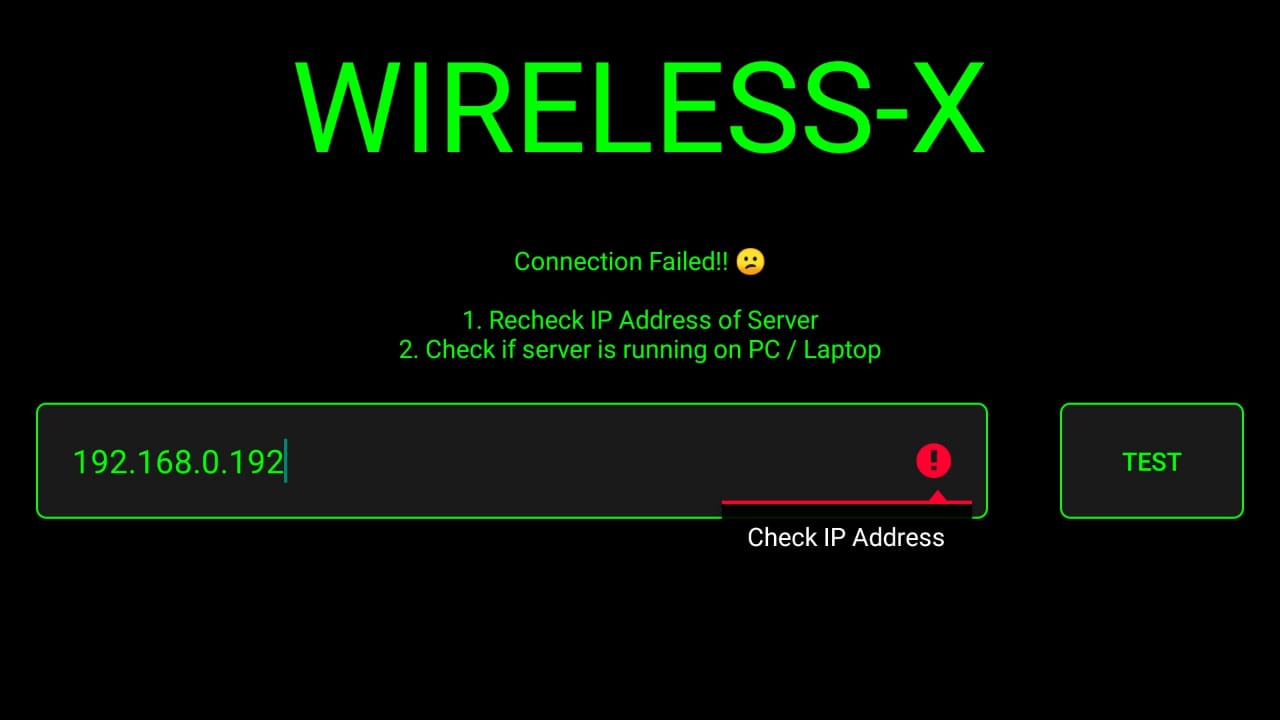
\includegraphics[scale=0.25]{images/connectionFailed.jpeg}
\end{center}
\item (Skip this step if connection was successful) Before retrying to connect, make sure that you are entering correct IP, both mobile and laptop are on same network, your app has all the required permissions. If all this is working fine, please try restarting your server and app and try again.
\item After successfully connecting to your laptop, click on \textbf{Enter Wireless-X} button. 
\item Now you have to select the mode you want to use. You can choose mouse mode by selecting button above it. Your screen should look like:
\begin{center}
    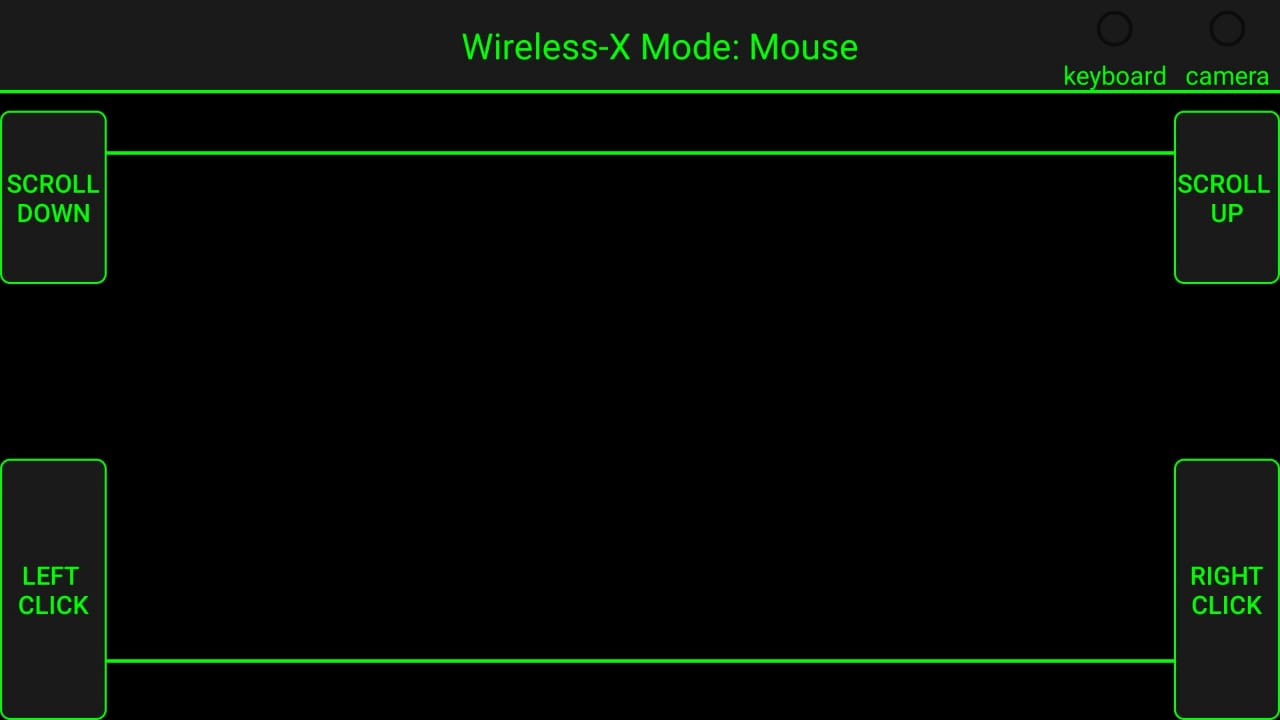
\includegraphics[scale=0.25]{images/mouse.jpeg}
\end{center}
Central part of your screen will be used to move mouse pointer. \textbf{Left click} and \textbf{Right click} button do their respective jobs of selecting things or giving more options menu. \textbf{Scroll Up} and \textbf{Scroll Down} buttons do the job of scroll wheel.
\item You can use Mouse mode along with Web-cam by selecting button above the option. As soon as you select this, you will see one more button to switch between front and back camera to substitute as your webcam. Below is a reference image where you can see camera feed being rendered on top-left corner. Same will be rendered to your laptop:
\begin{center}
    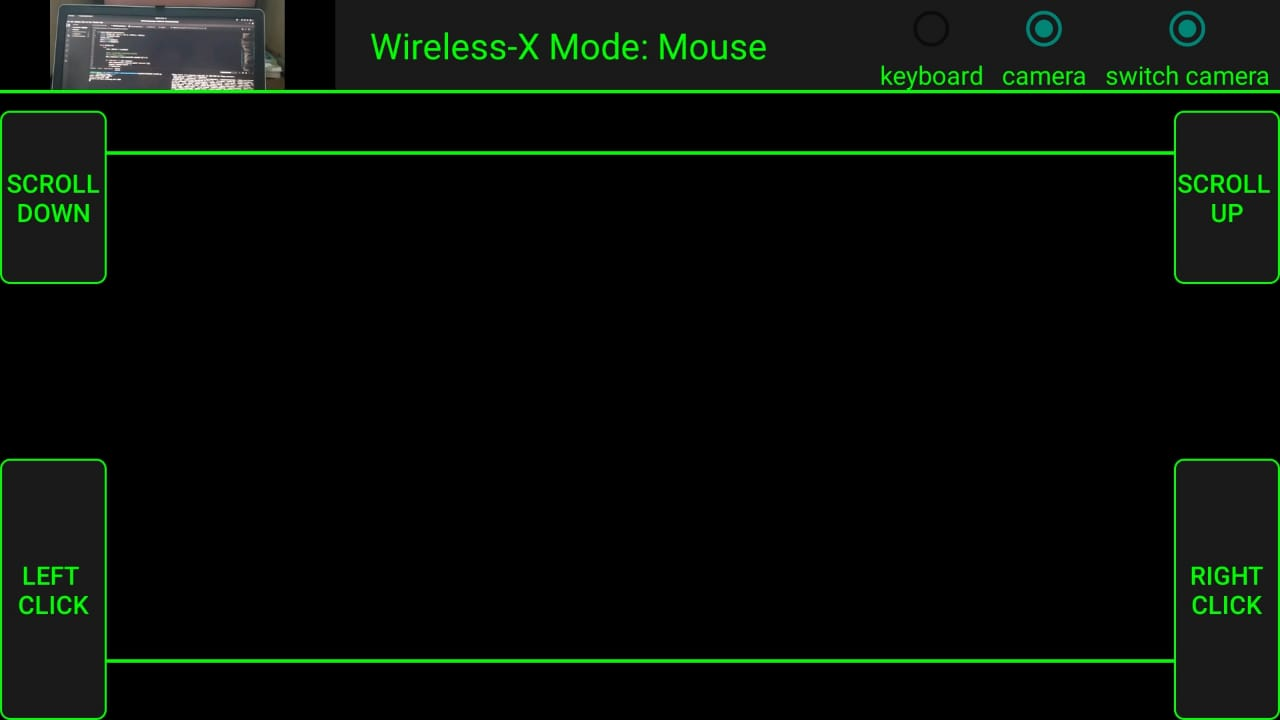
\includegraphics[scale=0.25]{images/mouseCamera.jpeg}
\end{center}
\item Now you can switch to keyboard mode by selecting button above it. Your screen should look like:
\begin{center}
    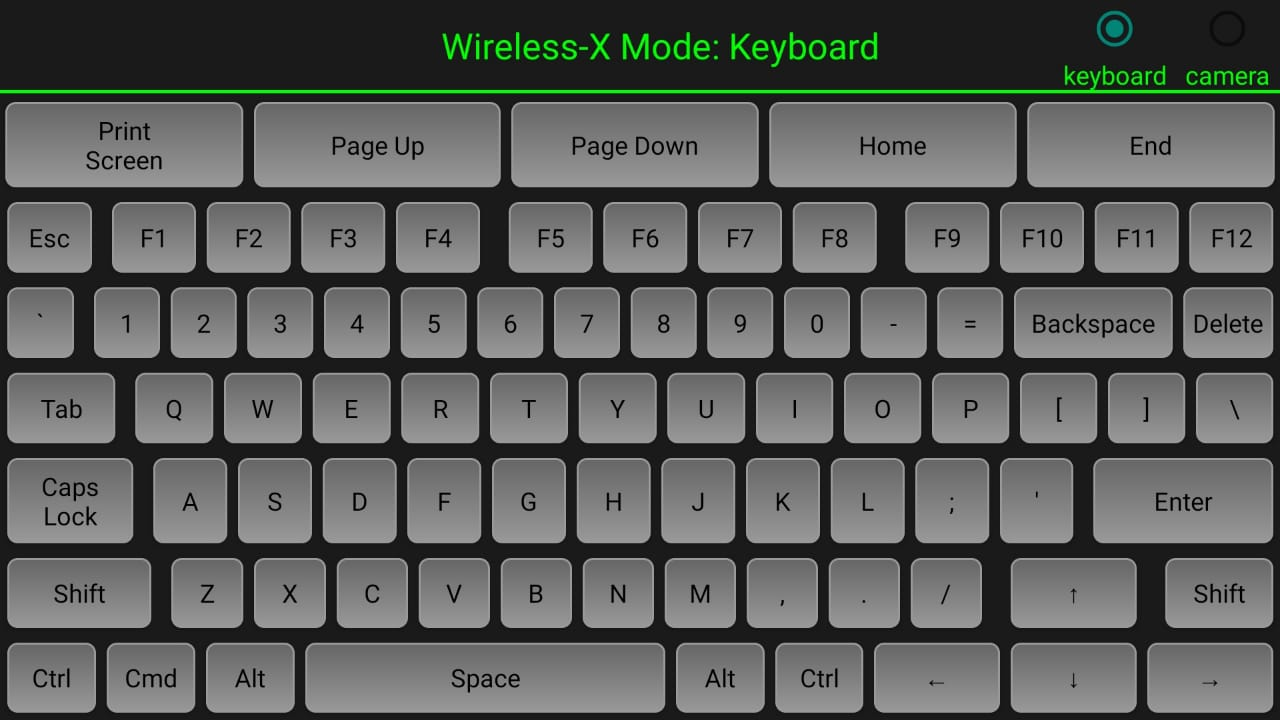
\includegraphics[scale=0.25]{images/keyboard.jpeg}
\end{center}
As you can see, this is a custom made keyboard layout since all the buttons of a physical keyboard are not present in smartphone's keyboard.
\item As with the mouse, you can use Keyboard mode along with Web-cam by selecting button above the option. As soon as you select this, you will see one more button to switch between front and back camera to substitute as your webcam. Below is a reference image where you can see camera feed being rendered on top-left corner. Same will be rendered to your laptop:
\begin{center}
    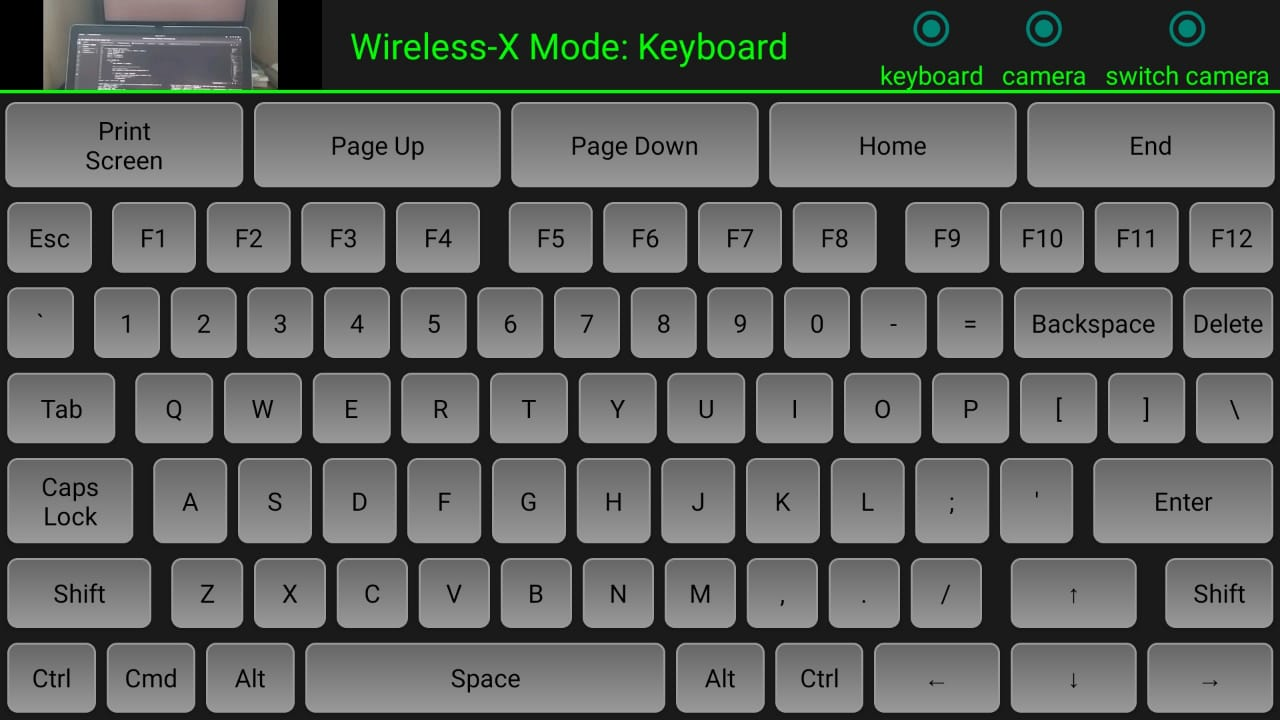
\includegraphics[scale=0.25]{images/keyboardCamera.jpeg}
\end{center}
\item This virtual keyboard also emulate the effect of "Shift" button being used along with other characters. For example, Shift + 1 gives '!' symbol. So, as soon as you click "Shift", you will see that all corresponding keys will be highlighted with the symbol it will generate on a physical keyboard and you can use those symbols too. Below is a reference image:
\begin{center}
    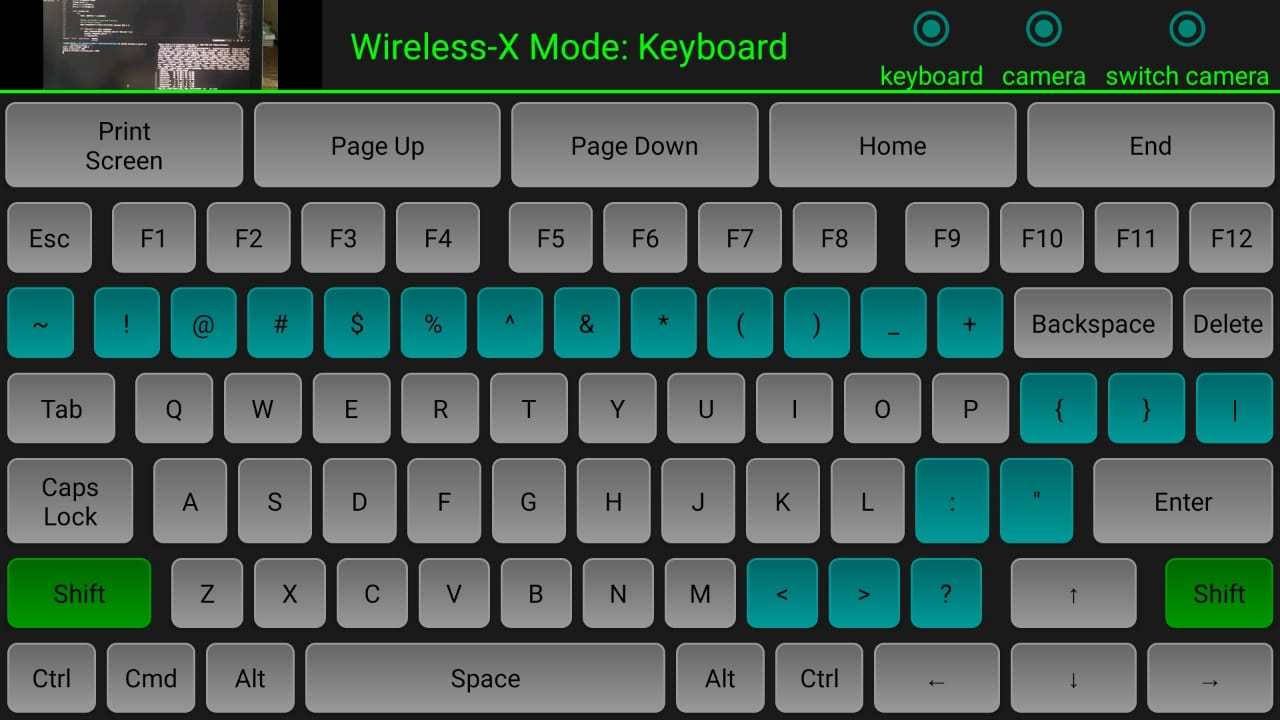
\includegraphics[scale=0.25]{images/shift.jpeg}
\end{center}
\item It can also emulate the effect of "Caps Lock" as well. Click on "Caps Lock". If you have a light to indicate Caps Lock being enabled or disabled in your physical keyboard, you can observe it being toggled by Wireless-X's keyboard. To show Caps Lock is enabled, as soon as you enable it, Caps Lock button will change color. Below is a reference image:
\begin{center}
    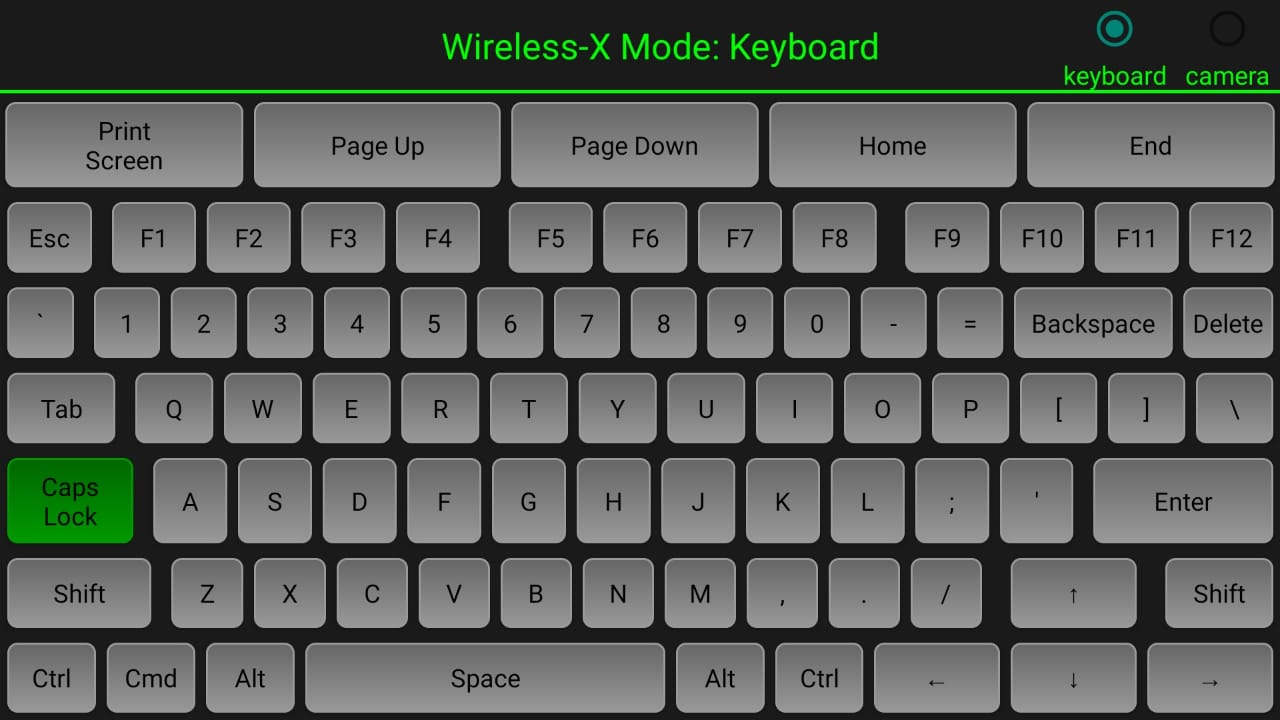
\includegraphics[scale=0.25]{images/capsLock.jpeg}
\end{center}
\end{enumerate}

\end{document}

